The Higgs boson mass dependent signal selections in the cut-based analysis 
are described in Section~\ref{sec:anal_cutbased}. In this section we summarise 
the results obtained all jet final states. 
Tables~\ref{tab:yield_cutbased} shows the signal %equivalent data yields
and background expectations in ee and $\mu\mu$ final states.
The expected cross section ratio limits as a function of the Higgs mass, 
together with the 1/2-$\sigma$ uncertainty bands in Table~\ref{tab:limits_cutbased_5fb} and Figure~\ref{fig:limits_5fb}. 
The observed exclusion region for the Standard Model Higgs is [300,450]~\GeV{} at 95\%C.L., 
compared to the expected exclusion region as [300,475]~\GeV{} at 95\%C.L.


%%%%%%%%%%%%%%%%%%%%%%%%%
\begin{table}[!ht]
{\small
\begin{center}
 \begin{tabular}{l | c c |  c c c c c c | c }
 \hline\hline
 $m_H$ & qqH & ggH & qqZZ & ggZZ & WZ & WWTop & Zjets & $\sum$Bkg & Data \\
 \hline
\multicolumn{10}{c} {ee} \\ \hline
250 & $0.9\pm0.1$ & $8.2\pm1.2$ & $13.2\pm1.4$ & $1.2\pm0.3$ & $9.7\pm1.2$ & $29.4\pm3.6$ & $6.0\pm6.0$ & $59.5\pm6.3$ & 58 \\
300 & $0.9\pm0.1$ & $7.9\pm1.2$ & $8.7\pm0.9$ & $0.8\pm0.2$ & $5.3\pm0.7$ & $9.6\pm2.1$ & $3.0\pm3.0$ & $27.3\pm3.2$ & 20 \\
350 & $0.7\pm0.1$ & $8.0\pm1.3$ & $6.2\pm0.7$ & $0.5\pm0.1$ & $2.8\pm0.4$ & $0.9\pm0.7$ & $1.7\pm1.7$ & $12.2\pm1.9$ & 10 \\
400 & $0.5\pm0.1$ & $6.7\pm1.2$ & $4.6\pm0.5$ & $0.4\pm0.1$ & $1.9\pm0.3$ & $0.0\pm0.4$ & $1.0\pm1.0$ & $8.0\pm1.2$ & 7 \\
500 & $0.3\pm0.1$ & $2.9\pm0.7$ & $2.8\pm0.3$ & $0.2\pm0.0$ & $0.9\pm0.1$ & $0.0\pm0.4$ & $0.5\pm0.5$ & $4.4\pm0.6$ & 5 \\
600 & $0.2\pm0.1$ & $1.1\pm0.4$ & $1.4\pm0.2$ & $0.1\pm0.0$ & $0.4\pm0.1$ & $0.0\pm0.4$ & $0.3\pm0.3$ & $2.2\pm0.3$ & 0 \\
\hline
\multicolumn{10}{c} {$\mu\mu$} \\ 
\hline
250 & $1.3\pm0.1$ & $11.7\pm1.7$ & $19.6\pm1.9$ & $1.8\pm0.4$ & $14.4\pm1.7$ & $36.5\pm4.5$ & $8.6\pm8.6$ & $81.0\pm9.0$ & 82 \\
300 & $1.2\pm0.1$ & $11.2\pm1.6$ & $12.7\pm1.2$ & $1.1\pm0.2$ & $7.5\pm0.9$ & $11.7\pm2.5$ & $4.4\pm4.4$ & $37.4\pm4.6$ & 41 \\
350 & $1.0\pm0.1$ & $11.0\pm1.7$ & $8.5\pm0.8$ & $0.7\pm0.2$ & $4.3\pm0.5$ & $1.1\pm0.7$ & $2.6\pm2.6$ & $17.2\pm2.8$ & 17 \\
400 & $0.7\pm0.1$ & $9.4\pm1.6$ & $6.6\pm0.7$ & $0.5\pm0.1$ & $2.8\pm0.3$ & $0.0\pm0.4$ & $1.6\pm1.6$ & $11.6\pm1.8$ & 11 \\
500 & $0.4\pm0.1$ & $3.9\pm0.9$ & $4.2\pm0.4$ & $0.3\pm0.1$ & $1.2\pm0.2$ & $0.0\pm0.4$ & $0.8\pm0.8$ & $6.5\pm0.9$ & 9 \\
600 & $0.2\pm0.1$ & $1.5\pm0.5$ & $2.2\pm0.2$ & $0.2\pm0.0$ & $0.5\pm0.1$ & $0.0\pm0.4$ & $0.3\pm0.3$ & $3.2\pm0.4$ & 5 \\
\hline\hline
\end{tabular}
\end{center}
}
\caption{Expected number of signal and background events for an integrated luminosity of \intlumi after applying the higgs selections 
  in the cut-based analysis in the ee final state. Both statistical and systematic uncertainties are included. 
For the sum of the $\ww$ and Top backgrounds, the uncertainties are modelled by a Gamma function of the number 
of $e\mu$ events in the control region.  }
\label{tab:yield_cutbased}
\end{table}

%%%%%%%%%%%%%%%%%%%%%%%%%%%%%%%
\begin{table}[!ht]
\begin{center}
\begin{tabular}{cccccc}
\hline\hline
Mass & Observed & Median Expected & [-$\sigma$, +$\sigma$] & [-2$\sigma$, +2$\sigma$]\\\hline
250 & 1.62 & 1.62 & [1.17, 2.24] & [0.88, 2.98] \\
300 & 0.95 & 1.04 & [0.75, 1.44] & [0.56, 1.91] \\
350 & 0.60 & 0.68 & [0.49, 0.94] & [0.37, 1.25] \\
400 & 0.59 & 0.65 & [0.47, 0.91] & [0.35, 1.21] \\
500 & 1.61 & 1.19 & [0.86, 1.66] & [0.65, 2.20] \\
600 & 2.20 & 2.36 & [1.70, 3.28] & [1.28, 4.36] \\
\hline\hline
\end{tabular}
\end{center}
\caption{The median expected cross section ratio limits as a function 
of the Higgs mass, together with the 1/2-$\sigma$ uncertainty bands obtained in the cut-and-count analysis, corresponding to 
an integrated luminosity of \intlumi}
\label{tab:limits_cutbased_5fb}
\end{table}

%%%%%%%%%%%%%%%%%%%%%%%%%%%%%
\begin{figure}[!htbp]
\begin{center}
   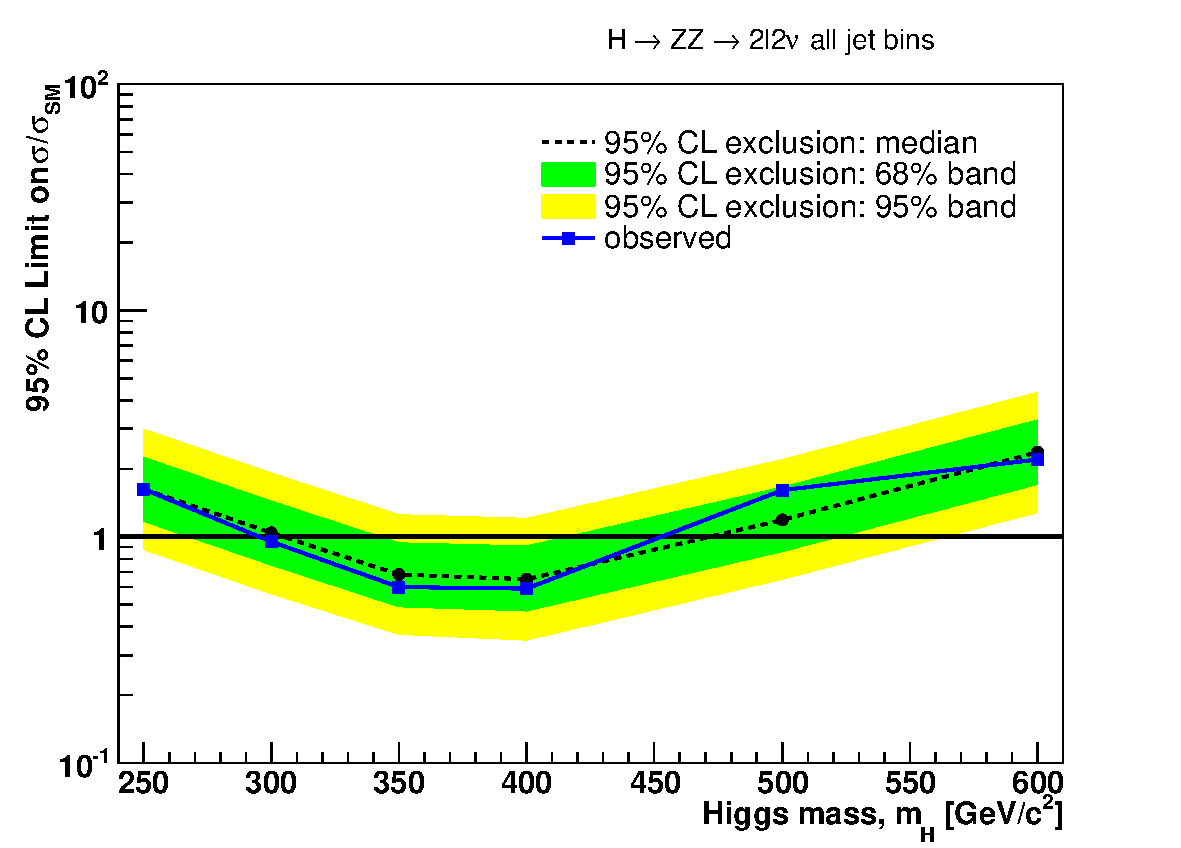
\includegraphics[width=0.8\textwidth]{figures/limits_cut_5fb.pdf}
   \caption{ The expected upper limits at 95\% C.L. for \intlumi\ of data for the cut-based analysis.}
   \label{fig:limits_5fb}
\end{center}
\end{figure}
%%%%%%%%%%%%%%%%%%%%%%%%%%%%%


\clearpage
